\documentclass[11pt, letterpaper, includehead]{article}

%%%%%%%%%%%%%%%%%%%%% Pre-document %%%%%%%%%%%%%%%%%%%%%
\usepackage{fancyhdr}  % Allow for headers
\usepackage{graphicx}  % Allow for figures 
\usepackage{float}     % Allow for figure inserted in specified location
\usepackage{amsmath}   % Allow for aligned math
\usepackage{array}     % Allow for cell width manipulation
\usepackage{nicematrix}
\usepackage{amssymb} % Uhhhh what was this????
\usepackage{multicol}

\setlength{\parindent}{0pt} % Remove auto paragraph indents

% Get rid of those big ass margins
\usepackage[margin=1in]{geometry}

% Table cell formatting
\setlength{\arrayrulewidth}{0.25mm}
\setlength{\tabcolsep}{11pt}
\renewcommand{\arraystretch}{1.2}

\begin{document}

%%%%%%%%%%%%%%%%%%%%% Title Page %%%%%%%%%%%%%%%%%%%%%
\begin{titlepage}
  \begin{center}
    \Huge{\textbf{Lab 8}}\\
    \Huge{Conservation of Energy}
    \vfill
    \begin{figure}[H] % H makes the figure insert at the position in the document
      \centering 
      \includegraphics[width=6cm]{../logo.png}
    \end{figure}
    \large{\textbf{your name here}}\\
    \large{Julian Barossi, Liam Gilligan, Stephanie L'Heureux}\\
    \vspace{0.5cm}
    \normalsize
    \today
  \end{center}
\end{titlepage}

%%%%%%%%%%%%%%%%%%%%% TABLE OF CONTENTS %%%%%%%%%%%%%%%%%%%%%
\tableofcontents
\pagebreak % Move to next page

% Add a nice fancy header
\pagestyle{fancy}
\fancyhead{}
\fancyhead[C]{\textbf{Lab 8:} Conservation of Energy}

\section{Mass-spring system} % 1
\subsection{Unstretched position and spring constant k}
\subsubsection{Unstretched position}
The unstreched length of the spring is defined as the spring's natural length when no forces
are applied to stretch or compress it. We recorded the position using the digits display 
of the motion sensor and found the value of the initial position ($x_0$) to be $0.67m$.

\subsubsection{Spring constant k}
The amount of force required to stretch or compress a spring a certain distance is defined by the spring constant $k$.
To find the value of $k$ we first measured the unstretched position of the spring
($x_0$) as discussed above. Then we added a hanger and mass totaling $100g$ to the spring and recorded the position
with the motion sensor. The stretched distance $x$ was found to be $0.39m$, and thus $\Delta x$ was $0.28 m$.\\

Because the hanger is at rest, the acceleration is zero, and thus the sum of the forces in the y
direction is zero. The weight of the hanging mass $mg$ acts downward and the force of the spring
($F_{sp}$) acts upward. In addition, note the force a spring exerts is defined by Hooke's law as $F_{sp} = -k \Delta x$. 
Using this information, $k$ is computed with the following calculations:
\begin{multicols}{2}
$$\Sigma F_y = ma_y$$
$$F_{sp} - mg = 0$$
$$F_{sp} = mg$$
$$F_{sp} = (0.100kg)(9.80m/s)$$
$$\boxed{F_{sp} = 0.980 N}$$

\columnbreak

$$F_{sp} = -k \Delta x$$
$$k = -\frac{F_{sp}}{\Delta x}$$
$$k = -\frac{0.980 N}{-0.28m}$$
$$\boxed{k = 3.5N/m}$$
\end{multicols}

\subsection{Setup and data taking}
\begin{center} 
  \begin{tabular}{| m{3cm} |  m{3cm} |} 
    \hline
     \textbf{Quantity} & \textbf{Value}\\ 
      \hline
      $x_0$ & $0.67m$ \\ 
      \hline
      $k$ & $3.5N/m$ \\ 
      \hline
      $m$ & $0.100kg$\\
      \hline
      $g$ & $9.8 m/s^2$\\
      \hline
  \end{tabular} 
\end{center}

\pagebreak

\subsection{Data analysis}
\textbf{Focus on one complete cycle of the mass-spring system and indicate 
on your plot the two turning points (lower and higher) and the equilibrium point.}\\

\begin{multicols}{2}
\begin{figure}[H] % H makes the figure insert at the position in the document
  \centering 
  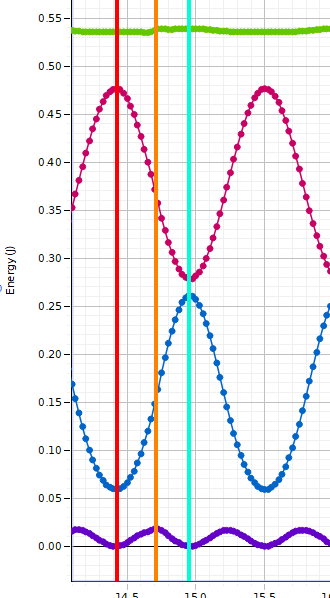
\includegraphics[width=2.5cm]{graph.png}
\end{figure}
\columnbreak

% Define colors 
\definecolor{purple}{RGB}{93, 63, 211}
\definecolor{green}{RGB}{76, 187, 23}

\begin{center} 
  \begin{tabular}{| m{1cm} |  m{1cm} | m{1cm} |m{1cm} |} 
    \hline
     \boldmath{$U_s$} & \boldmath{$U_g$} & \boldmath{$E_{tot}$} & \boldmath{$K$}\\ 
      \hline
      \Large\textcolor{blue}{\ensuremath\bullet} & \Large\textcolor{magenta}{\ensuremath\bullet} &  \Large\textcolor{green}{\ensuremath\bullet} & \Large\textcolor{purple}{\ensuremath\bullet}\\
      \hline
  \end{tabular} 
\end{center}
\end{multicols}


\textbf{Is $U_g$ is a minimum, a maximum, or neither? Explain why.}\\
\textbf{Is $U_{sp}$ is a minimum, a maximum, or neither? Explain why.}\\
\textbf{Is $k$ is a minimum, a maximum, or neither? Explain why.}\\

\textbf{Why does the kinetic energy curve peak twice per cycle?}\\
\textbf{Is mechanical energy conserved? Justify your answer with 
data. If not, can you identify (and possibly eliminate) systematic 
errors in your data?}\\
Mechanical energy is defined as the sum of potential and kinetic energy. 
For energy to be conserved, the change in energy $\Delta E$ must be 0 where 
$\Delta E$ is the sum of all energies in the system. The plot shows 

\section{Conservation of energy}
\subsection{Overview}
The law of conservation of energy states that in a system in which no work is done
($\Delta E = 0$) the total energy in the system is conserved. Energy may change forms 
within the system, however, because energy cannot be created or destroyed, the total energy is constant. In this experiment, we observe the law of conservation of energy as energy is 
converted from elastic potential energy ($U_{sp}$) to kinetic ($K$) and gravitational potential 
energy ($U_g$). The law of conservation of energy was used to predict the distance up an inclined track 
a cart will reach having been launched by a spring. This prediction can be made assuming there
is no work being done on the system. Therefore, gravitational potential energy ($U_g$) the cart has at its maximum height up the ramp 
may be found from the elastic potential energy in the spring upon launch. From $U_g$, the height ($h$) may be found
and by basic trigonometry, the distance traveled up the ramp may be calculated.

\subsection{Procedure}
\begin{enumerate} 
  \item Find the spring constant $k$ of the spring utilized by the cart launcher. 
  This may be accomplished by attaching the cart to the launcher and compressing the 
  spring a known distance. The carts are equipped with a force sensor, so from knowing the force 
  required to compress the spring a certain distance, k is computed.
  by attaching the string to a cart and using a force sensor.
  \item Position the track at an incline with the spring launcher at the bottom 
        and the motion sensor at the top. 
  \item Measure the angle of the incline by measuring the adjacent and opposite lengths
  then taking the $\arcsin$ to find $\theta$.
  \item Predict the distance the car will travel up the ramp using conservation of energy to find $\Delta x_{thy}$
  \item Run the experiment and collect 10 data points of $\Delta x_{exp}$.
  \item Calculate an average distance traveled along the ramp ($\bar{x}$) , standard deviation 
  ($\sigma$), and a standard error ($SE$).
  \item Is the theory ($x_{thy}$) consistent with experiment ($x_{exp}$)?
\end{enumerate}

\subsection{Data}
The following table displays data collected from ten trials of the experiment. The first column \emph{Attempt} defines the experiment trial number. \emph{Distance (x)}
is the actual distance in meters traveled up the ramp by the cart. This is the main focus of the experiment. 
We also wanted to verify conservation of energy, so we also computed the vertical height traveled by the cart and used this to 
calculate the gravitational potential energy. This data is represented in columns \emph{Height (h)} and \emph{$U_g$}, respectively. 
\begin{center} 
  \begin{tabular}{|  m{2cm} | m{3cm} | m{3cm} | m{3cm} | } 
    \hline
    \textbf{Attempt} & \textbf{Distance ($x$)} & \textbf{Height ($h$)} & \boldmath{$U_g$} \\ 
    \hline
    1 & 0.190 & 0.032 & 0.095 \\ 
    \hline
    2 & 0.179 & 0.030 & 0.089 \\ 
    \hline
    3 & 0.171 & 0.029 & 0.085 \\ 
    \hline
    4 & 0.181 & 0.031 & 0.090 \\ 
    \hline
    5 & 0.179 & 0.030 & 0.089 \\ 
    \hline
    6 & 0.177 & 0.030 & 0.088 \\ 
    \hline
    7 & 0.168 & 0.029 & 0.084 \\ 
    \hline
    8 & 0.177 & 0.030 & 0.088 \\ 
    \hline
    9 & 0.165 & 0.028 & 0.082 \\ 
    \hline
    10 & 0.176 & 0.030 & 0.088 \\ 
    \hline
  \end{tabular} 
\end{center}

The distance traveled up the ramp by the cart ($x$), was the value of interest in this experiment, the following 
table displays statistical data for this quality. 

\begin{center} 
  \begin{tabular}{|  m{3cm} | m{3cm} | } 
    \hline 
    \textbf{Quantity} & \textbf{Value}\\
    \hline
    Average ($\bar{x}$) & 0.176  \\ 
    \hline
    STDEV ($\sigma$)& 0.007\\ 
    \hline
    $SE$ & 0.002\\ 
    \hline      
  \end{tabular} 
\end{center}

\subsection{Data analysis}
\subsubsection{Prediction}
% Add finding k
The spring constant $k$ is required for future calculations. To find the value of $k$, we needed to know the distance
the spring compressed when applying some force. The carts have a force sensor which means we can attach the spring to the cart and press 
on the force sensor to determine how much force is applied to the spring. When that force is applied, the distance the spring was 
compressed can also be measured. With these two qualities, force and a compression distance, the spring constant for the spring may be computed as follows
$$k = \frac{F}{\Delta x}$$
$$k = \frac{2.86 N}{0.025m}$$
$$\boxed{k = 114.4N/m}$$


We will look at the energy at the bottom of the track when the cart is launched by 
the spring and compare it to the energy of the cart at its highest point along the incline.
$$\Delta E = \Delta K + \Delta U_{g} + \Delta U_{sp} + \Delta E_{th} + \Delta E_{chem}$$
Assuming there is no friction, there is no work done on the system and thus
the equation becomes 
$$0 = \Delta U_{g} + \Delta U_{sp}$$
$$(U_{g})_i + (U_{sp})_i = (U_{g})_f + (U_{sp})_f$$
$$(U_{sp})_i = (U_{g})_f$$
$$\frac{1}{2}k\Delta x^2 = mgh$$
$$h = \frac{k\Delta x^2}{2mg}$$
$$h = \frac{(114.4 N/m) (0.025m)^2}{2 (0.2996kg)(9.80m/s^2)}$$
$$\boxed{h = 0.0122m}$$

From the predicted vertical height traveled using trigonometry, the distance up the ramp may be found.
First to find the angle of the incline, the opposite and adjacent sides of the track were measured. Then
the $\arcsin$ was taken.

\begin{center} 
  \begin{tabular}{|  m{3cm} | m{3cm} | } 
    \hline 
    \textbf{Quantity} & \textbf{Value}\\
    \hline
    Adjacent & $90cm$ \\ 
    \hline
    Opposite & $15.5cm$ \\ 
    \hline
    Angle ($\theta$) & $9.7717^{\circ}$ \\ 
    \hline      
  \end{tabular} 
\end{center}

The predicted distance traveled by the cart along the ramp could then be
found by 
$$x_{thy} = \frac{h}{\sin \theta}$$
$$x_{thy} = \frac{0.0122m}{\sin(9.7717^{\circ})}$$

\subsubsection{Theory vs experinent}
$$x_{exp} \pm 2SE$$
$$0.1763m \pm 2(0.00223631641569593m)$$
$$0.1763m \pm 0.0044726328313919m$$
$$x_{thy}\in [0.1718273671686081 s, 0.1807726328313919m]$$
$$\in [0.1718273671686081 s, 0.1807726328313919m]$$
The 

\subsection{Conclusion}

\end{document}